\textbf{Binomials}
\fbox{\begin{minipage}{0.31\textwidth}
\begin{align*}
&	\sum_{k = 0}^{n} C_n^k = 2^n 
&	\sum_{k = 0}^{m} C_{n + k}^k = C_{n + m + 1}^m \\
&	\sum_{m = 0}^{n} C_m^k = C_{n + 1}^{k + 1} 
&	\sum_{k = 0}^{n} (C_n^k)^2 = C_{2n}^n \\
&	\sum_{j = 0}^{k} C_m^j C_{n-m}^{k - j} = C_n^k 
&	\sum_{j = 0}^{m} C_m^j C_{n-m}^{k - j} = C_{n + 1}^{k + 1} \\
&	\sum_{k = 0}^{n} C_{n - k}^k = F_{n + 1}
\end{align*}
\end{minipage}}

\textbf{Catalan}
\fbox{\begin{minipage}{0.31\textwidth}
\begin{align*}
& C_n = \sum_{k = 0}^{n - 1} C_kC_{n - 1 - k} = \frac{1}{n + 1} C_{2n}^{n} = C_{2n}^{n} - C_{2n}^{n - 1}\\
& 1, 1, 2, 5, 14, 42, 132, 429, 1430, 4862, 16796, 58786
\end{align*}
\end{minipage}}

\textbf{Fibonacci}
\fbox{\begin{minipage}{0.31\textwidth}
\begin{align*}
& F_1 = F_2 = 1 
& F_{n + k} = F_k F_{n + 1} + F_{k - 1} F_n \\
& F_n = F_{n - 1} + F_{n - 2} 
& F_{n + 1} F_{n - 1} - F_n^2 = (-1)^n \\
& gcd(F_m, F_n) = F_{gcd(n, m)} 
& F_{47} \approx 2.9e9\\
& F_n = \frac{(\tfrac{1 + \sqrt{5}}{2})^n - (\tfrac{1 - \sqrt{5}}{2})^n}{\sqrt{5}}
& F_{88} \approx 1.1e18
\end{align*}
\end{minipage}}

\textbf{Stirling}

$S(n, k)$ --- number of ways to divide $n$ element into $k$ non-empty groups.\\

$S(n, n) = 1$, $n \ge 0$\\
$S(n, 0) = 0$, $n > 0$\\

$S(n, k) = S(n - 1, k - 1) + S(n - 1, k) * k$.


$B_n = \sum S(n, k)$ from $n = 0$:

1, 1, 2, 5, 15, 52, 203, 877, 4140, 21147, 115975, 678570, 4213597, 27644437, 190899322, 1382958545, 10480142147, 82864869804,...


\subsection{Graphs}

\textbf{Prufer sequence}\\
The Prufer sequence of a labeled tree is unique and has length $n - 2$. 
At step $i$, remove the leaf with the smallest label and set the $i$-th 
element of the Prufer sequence to be the label of this leaf's neighbour.

\textbf{Spanning trees of a complete graphs}\\
For $K_n$ number of spanning trees is equal to $n^{n - 2}$.\\
For $K_{L, R}$ number is equal to $L^{R - 1} \cdot R^{L - 1}$.

\textbf{Cayley's theorem}\\
Let $T_{n, k}$ be the number of labelled forests on $n$ vertices with $k$ connected components, 
such that vertices $1, \dots, k$ all belong to different components. 
$T_{n,k} = k \cdot n^{n - k - 1}$.

\textbf{Spanning trees with fixed degrees}\\
The number of spanning trees in a complete graph $K_{n}$ with a fixed degrees
$d_{i}$ is equal to:
$ \frac{(n - 2)!}{\prod(d_i - 1)} $

\textbf{Spanning trees from forests}\\
For a forest graph with connected components of sizes $sz_0, \dots, sz_{k - 1}$, 
the number of ways to add edges to make a spanning tree is equal to:
$ n^{k - 2} \cdot \prod sz_i$

\textbf{Hook length formula}
A Young tableau is a filling of the $n$ cells of the Young diagram with a permutation, 
such that each row and each column form increasing sequences. 
The \textbf{hook} $h_{\lambda}(i, j)$ is number of cells $(a, b)$ in diagram such that
$a = i$ and $b \ge j$ or $a \ge i$ and $b = j$.


\fbox{
\noindent
\begin{minipage}{0.07\textwidth}
Number of tableaux:\\
$$\frac{n!}{\prod h_{\lambda}(i, j)}$$   
\end{minipage}
}
\hfill
\fbox{
\begin{minipage}{0.06\textwidth}
Tableaux:
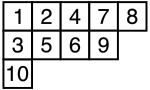
\includegraphics[width=\textwidth]{content/math/young-tableaux.png}
\end{minipage}
}
\hfill
\fbox{
\begin{minipage}{0.06\textwidth}
Hooks:
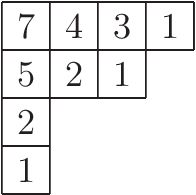
\includegraphics[width=\textwidth]{content/math/hook-length-tableau.jpg}
\end{minipage}
}

\textbf{\large{Chromatic polynomial}}\\
For a graph $G$, $\chi(G, \lambda) = \chi(\lambda)$ counts the number of coloring vertices in $\lambda$ colors.
There is a unique polynomial $\chi(\lambda)$. Deletion-contraction:
\begin{itemize}
\item The graph $G/uv$ is obtained by merging $u$ and $v$ into one. 
\item The graph $G - uv$ is obtained by deleting edge $uv$.
\item $\chi(G, \lambda) = \chi(G - uv, \lambda) - \chi(G/uv, \lambda)$. 
\end{itemize}

\begin{tabular}{|c|c|}
\hline
$G$ is tree & $\chi(\lambda) = \lambda(\lambda - 1)^{n - 1}$ \\
\hline
$G$ is cycle $C_n$ & $\chi(\lambda) = (\lambda - 1)^n + (-1)^n(\lambda - 1)$\\
\hline
\end{tabular} 
 
\textbf{Proposition 1} $\chi(\lambda)$ is equal to the number of pairs $(\sigma, O)$, 
where $\sigma$ is any map $\sigma : V \rightarrow \{1, \dots, \lambda\}$ and $O$ is an orientation of $G$, 
subject to the two conditions:
\begin{itemize}
\item The orientation $O$ is acyclic.
\item If $u \rightarrow v$ in $O$, then $\sigma (u) > \sigma (v)$.
\end{itemize}

\textbf{Proposition 2} Define $\overline{\chi}(\lambda)$ to be the number of pairs $(\sigma, O)$, 
where $\sigma$ is any map $\sigma : V \rightarrow \{1, \dots, \lambda\}$ and $O$ is an orientation of $G$, 
subject to the two conditions:
\begin{itemize}
\item The orientation $O$ is acyclic.
\item If $u \rightarrow v$ in $O$, then $\sigma (u) \ge \sigma (v)$.
\end{itemize}

\textbf{Proposition 3} Suppose that $|V| = n$. Then for all non-negative integers $\lambda$ holds:
$$\overline{\chi}(\lambda) = (-1)^n \chi(-\lambda)$$


$\overline{\chi}(1)$ is number of ways to orient edges to make a DAG.
